\usepackage{here}
\usepackage{ascmac}
\usepackage{here}
\usepackage{txfonts}
\usepackage{listings, jlisting}
\renewcommand{\lstlistingname}{リスト}
\lstset{
  basicstyle=\ttfamily,
  commentstyle=\textit,
  classoffset=1,
  keywordstyle=\bfseries,
  frame=single,
  framesep=5pt,
  showstringspaces=false,
  numbers=left,
  stepnumber=1,
  numberstyle=\tiny,
  tabsize=2,
  breaklines=true
}



\title{SNS経由で入手される情報のユーザ間差異の可視化}
\author{プロジェクトマネジメントコース\\
ソフトウェア開発管理グループ\\
矢吹研究室\\
1242131\\
吉野 聡志}
\date{}
\begin{document}
\maketitle

\chapter*{謝辞}

\tableofcontents%目次

\chapter{序論}

\section{論文構成}
本稿では以下のような構成をとる.・・・

\chapter{背景}
世界的に人気のあるSNS(Social Networking Service)のひとつとしてTwitter が存在する.2015年6月30日現在,月間アクティブユーザは3億1600万人である.SNSの中でもアクティブユーザ数が非常に多く,利用スタイルも多数あるTwitter に対し,ユーザである人々が顕在的・潜在的に持っているニーズが何であるかが分かれば,他のSNS(Facebook等)との差別化を図りやすくなる.これにより効率的なマーケティングの手法をTwitter社や,Twitter上に広告を打ち出す企業に提案できるのではないか,と考えられる.

\chapter{目的}

\section{目的}
後述する方法で数名のTwitterタイムラインを取得し,各人のタイムライン上に並ぶ単語や,単語同士の結びつきの強さを可視化する.その結果からつぶやきの性質を分析し,各人の嗜好や関心事項と合致するもの・しないものを見つけ出し,Twitterへの顕在的・潜在的なニーズを読み取ることが目的である.

\section{プロジェクトマネジメントとの関連性}
・・・

\chapter{手法}

\section{本章の構成}
本章では,本研究で利用するTwitterの機能や,研究を行うための環境設定・利用するサービスについて解説したのち,研究の手法について記す.

\section{Twitterとは}
Twitterは,つぶやきと呼ばれる短い発言を投稿し,他のユーザが閲覧・返信することによってコミュニケーションが生まれるSNSである.他のユーザのつぶやきを追跡することを「フォローする」という.タイムラインと呼ばれる画面には,自分のつぶやきとフォローしたユーザのつぶやきが同一画面上に,リアルタイムで表示される.相手がつぶやきを非公開にしていなければ,フォローをする際の承認は不要で,つぶやきを引用することもできる.つぶやきやユーザの検索をすることも可能で,ユーザ同士がつながる機会は多岐にわたる.

\begin{figure}[H]
\centering
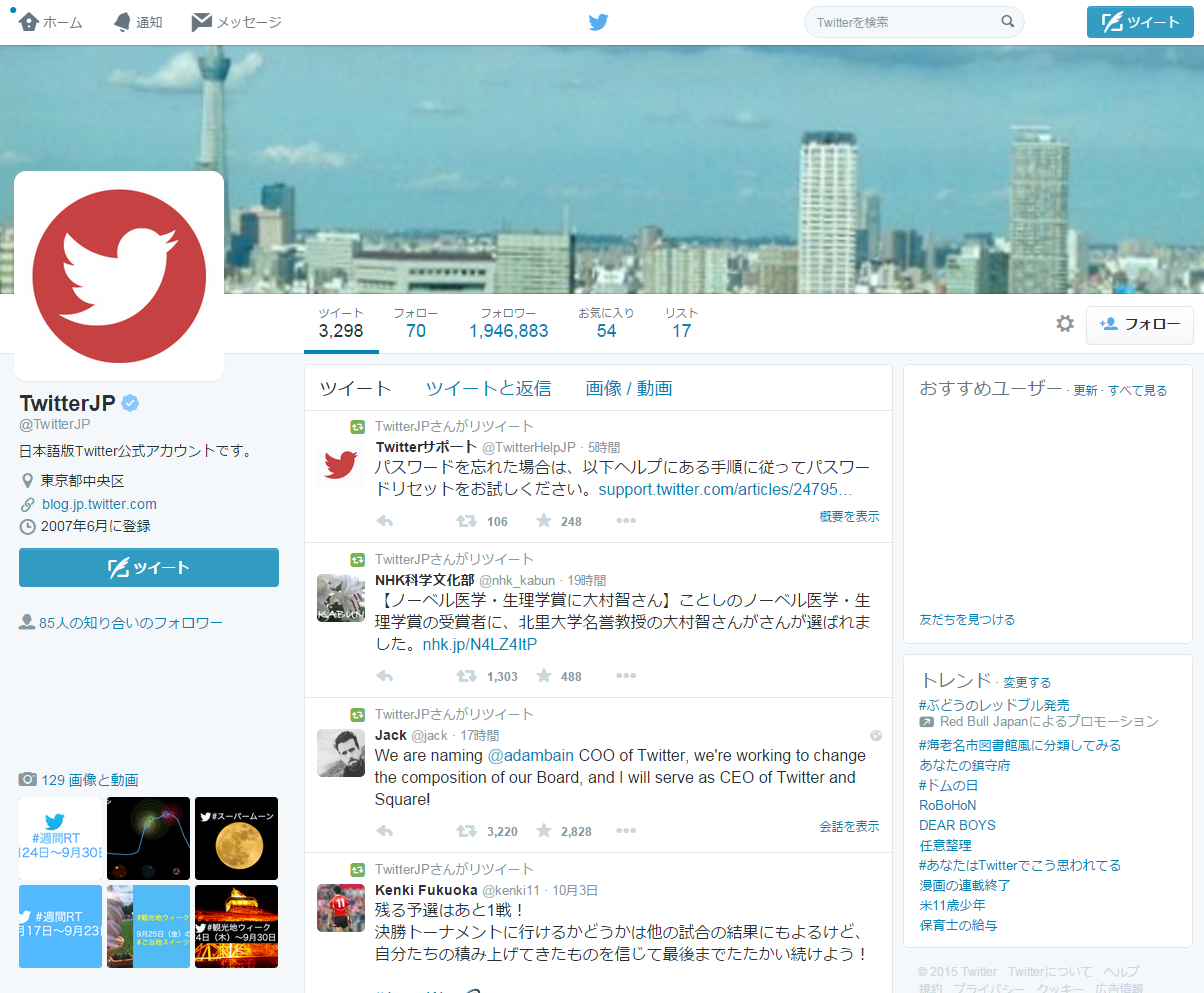
\includegraphics[width=15cm]{TwitterJP.png}
\caption{日本語版Twitter公式アカウントのプロフィール画面}\label{TwitterJP}
\end{figure}

\section{用語}
本節では,本研究で利用するTwitterの用語について説明する\cite{twitterwords}.

\subsection{スクリーンネーム}
ユーザがアカウントを登録する際,ユーザ同士を区別するために設定する名前.最大15文字の半角英数字とアンダースコアの組み合わせからなる.スクリーンネームの先頭には@が付く.登録した後,ユーザによる変更が可能.

\subsection{ユーザID}
ユーザがアカウントを登録する際,Twitterがユーザを識別するために決定する数字の羅列.スクリーンネームとは異なり,登録した後の変更は不可能.

\subsection{名前}
ユーザのプロフィールページでスクリーンネームとともに表示される名前.スクリーンネームと違い,日本語や記号を入れることができ,他のユーザとの重複があってもそのまま登録できる.登録後のユーザによる変更が可能.

\subsection{ツイート}
Twitterにおける「つぶやき」のこと.1つのツイートにつき160文字まで,という制限が設けられている.ただし,そのうちの20文字はユーザIDに割り当てられているため,残りの140文字がツイートの本文ということになる.

\subsection{タイムライン}
自分とフォローしているユーザのツイートがリアルタイムに,時系列に沿って表示される画面.この画面がTwitterでは基本となるため,「ホーム」とも呼ぶ.

\subsection{フォロー}
特定のユーザのツイートをタイムラインに表示するための操作.

\subsection{フォロワー}
特定のユーザをフォローしているユーザを指す.ユーザAがユーザBをフォローしている場合,ユーザAはユーザBのフォロワーである.

\subsection{リプライ(返信)}
特定のスクリーンネームから始まるツイート.そのユーザ宛のツイートということになる.

\subsection{リツイート}
他のユーザのツイートを,自分のフォロワーに向けてツイートする操作.

\subsection{お気に入り}
他のユーザのツイートを,自分のお気に入りリストへ登録する操作.

\subsection{メンション}
特定のスクリーンネームを含むツイート.リプライと違い,ツイート内のどこにスクリーンネームが入っていてもメンションとなる.非公式クライアントの種類によっては自分のスクリーンネームが入ったメンションを表示する機能がある.

\subsection{アクティビティ}
自分がフォローしているユーザが他のユーザをフォローしたり,ツイートをお気に入りに登録した等の活動履歴を一覧で表示するページ.フォロー相手の行動をリアルタイムで確認できるため,タイムラインの閲覧だけでは得られない新たな発見の可能性を生み出している.

\subsection{リスト}
ユーザをグループにまとめ,管理する機能.リストごとにタイムラインを表示させることができる.

\subsection{ハッシュタグ}
ツイート内に記載された\#から始まる文字列.ハッシュタグを付けてツイートするとその部分が自動的にリンクとなり,クリックすると同じタグが付いたツイートの検索結果が時系列で表示される.

\subsection{トレンド}
Twitter上のツイートの中で多く話題に上っているキーワードをリアルタイムに抽出し,表示する機能.表示するトレンドの地域を設定でき,全世界のトレンドを表示することもできる.

\subsection{短縮URL}
ツイートの文字数をURL含め140字以内に抑えるため,長いURLを短いURLに変換したもの.代表的なものとしてTwitter公式(http://t.co)がある.

\subsection{非公開ツイート}
フォロワーにのみツイートを公開する設定.非公開ツイートを設定しているユーザのツイートを閲覧するには,その相手に対しフォローリクエストを送信し,許可を得ることが必要となる.

\subsection{認証済みアカウント}
有名人等,多くの人に検索されたり,なりすましの対象になりうるユーザのTwitterアカウントについて,Twitter社が本人確認を行ったアカウント.認証済みアカウントにはプロフィール画面等にチェックマークの入ったブルーの認証バッジが表示される.

\section{Twitter APIについて}
本研究ではTwitterから様々な情報を取得するためのプログラムを使用する.その際に必要となるのがTwitter APIである.本節では,Twitter APIに関する説明をする.

\subsection{API}
アプリケーションプログラムインターフェイス(Application Program Interface)の略で,プログラミングの際に使用できる命令や規約,関数等の集合・枠組みのこと.ソフトウェア開発の際,一からすべてを作るには膨大な時間を要するが,APIという枠組みを利用することにより,プログラミングの負担を軽減することができる\cite{whatsapi}.

\subsection{Twitter API}
Twitter社が提供するAPI.これを利用することでWebサイトやアプリケーションなどからTwitterの機能を呼び出すことができ,ツイートの参照や検索等を行えるアプリケーション開発を行えるようになる\cite{whatstwitterapi}.

\subsection{REST API}
Twitter APIのパラメータ(リソース)を指定し,特定のURLにHTTPでアクセスすると,JSON形式で記述されたメッセージがレスポンスされるシステムのこと.これはツイートの更新や参照を行う際に使用する基本的なAPIとなる.ただし利用制限があり,15分以内に同じ機能を特定の回数利用すると,はじめにその機能を利用した時間から15分経過するまではその機能が利用できなくなる.

\subsection{Streaming API}
今回利用するAPI.タイムラインの変更をリアルタイムに受け取ることができる.REST APIと異なり,利用制限は設けられていない.

\subsection{Access Token}
Twitterに限らず,多くのユーザアカウントに存在するIDとパスワードのような「Access Token」と「Access Token Secret」の2種類の文字列を指す.これは,アプリケーションがユーザの代わりにユーザデータにアクセスするための「通行許可証」のようなものといえる.悪意ある第三者にIDとパスワードそのものを預けた場合,勝手にログインされたり,最悪の場合アカウントを削除することも可能となってしまう.そういったリスクを防ぐため,限られた範囲でユーザデータにアクセスできる権限としてAccess Tokenが利用される\cite{whatsAccessToken}.

\section{Oracle VM VirtualBoxとは}
Oracle VM VirtualBox(以下,VirtualBoxと表記する)は,使用しているPCマシン上に仮想的なマシンを作成し,別のOSをインストール・実行することができるオープンソースソフトウェアである.WindowsやMac OS X,Linux等,様々なOSで利用することができる\cite{VBoxMania}.

\section{用語}
本節では,本研究で利用するVirtualBoxの用語について説明する.

\subsection{ホストマシン(物理マシン)}
物理的に存在するコンピュータ.

\subsection{ホストOS}
ホストマシンにインストールされているOS.VirtualBoxはホストOSにインストールされる.本研究で使用するホストマシンのOSはWindows 7/8.1である. 

\subsection{バーチャルマシン(仮想マシン)}
VirtualBoxが作成する論理的なマシン.VirtualBoxがホストマシンのコンピュータ資源(CPUやメモリ,HDD等)の一部を仮想化し,ゲストマシンに割り当てる.ホストマシンの資源を使いきらない限り,ゲストマシンを複数作成したり,多重起動させることができる.

\subsection{ゲストOS(仮想OS)}
ゲストマシンにインストールされるOS.本研究では,Linuxディストリビューションの一つであるUbuntuをインストールした.

\subsection{仮想ディスク}
ゲストマシンが使用する仮想のハードディスク.バーチャルマシンからはこれを物理ディスクとして扱うことができる.仮想ディスクの実体はホストマシン内にファイルとして存在する.

\subsection{キャプチャ}
Guest Additions(後述)をインストールしていない状態でゲストOSの画面をクリックした際,キーボードやマウスの入力がゲストOSの中でしかできなくなってしまう状態.ホストキー(初期状態では右側のCtrlキー)を押す度に入力先をホストOSとゲストOSに切り替えられるが,その手間を省く等の理由でGuest Additionsをインストールする.

\subsection{Guest Additions}
VirtualBoxの操作性を向上させるためのモジュール.ホストOSとゲストOS間のシームレスなマウスポインタの移動や,ゲストOSの画面の解像度を自由に変更することなどが可能となる\cite{LinuxMania}.これはゲストOSにインストールするため,ゲストマシンごとにインストール作業をする必要がある.

\section{研究の手法}
\begin{description}
 \item[VirtualBoxのインストール]\mbox{}\\
 	http://www.oracle.com/technetwork/server-storage/virtualbox/downloads/index.htmlよりインストーラをダウンロードし,インストーラの指示に従ってVirtualBoxをインストールする.
 	
 \item[Ubuntuのインストール]\mbox{}\\
	まず,https://www.ubuntulinux.jp/download/ja-remixよりUbuntu 14.04のISOイメージをダウンロードする.本研究では64bit版を選択した.\\
	次にインストールしたVirtualBoxを立ち上げ,ウインドウ左上にある「新規(N)」のボタンを押してゲストマシンの作成を行う.\\
	ゲストマシンの名前,メモリサイズ,HDDの設定をするとウィンドウが閉じられる.
	
	\begin{figure}[H]
	\centering
	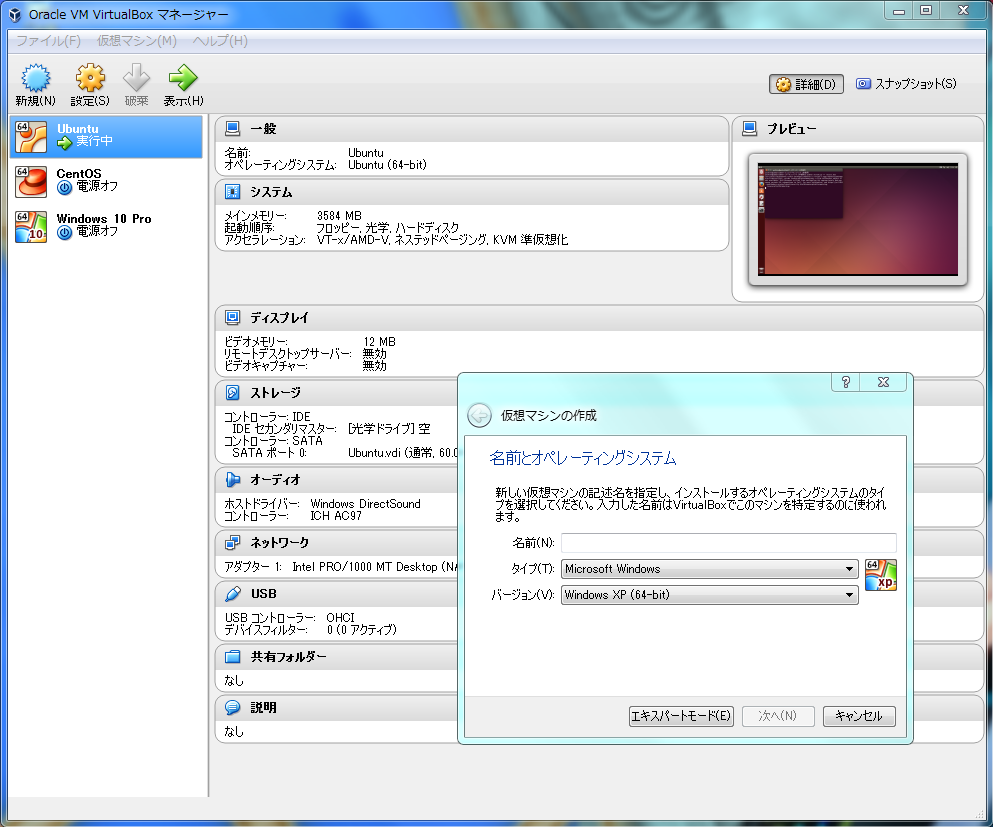
\includegraphics[width=15cm]{VBoxWindow.PNG}
	\caption{VirtualBoxのウィンドウとゲストマシン作成ウィンドウ}\label{VBoxSetup}
	\end{figure}
	
	続いて「設定(S)」を開き,「ストレージ」の項目にあるストレージツリーより,「コントローラー: IDE」内の「空」を選択する.\\%Ubuntuを利用していない時に詳細な説明を書いておく
	「属性」内にあるディスクのマークをクリックしてプルダウンメニューを開き,「仮想光学ディスクファイルを選択...」をクリックしてダウンロードしたISOイメージをマウントする.
	
	\begin{figure}[H]
	\centering
	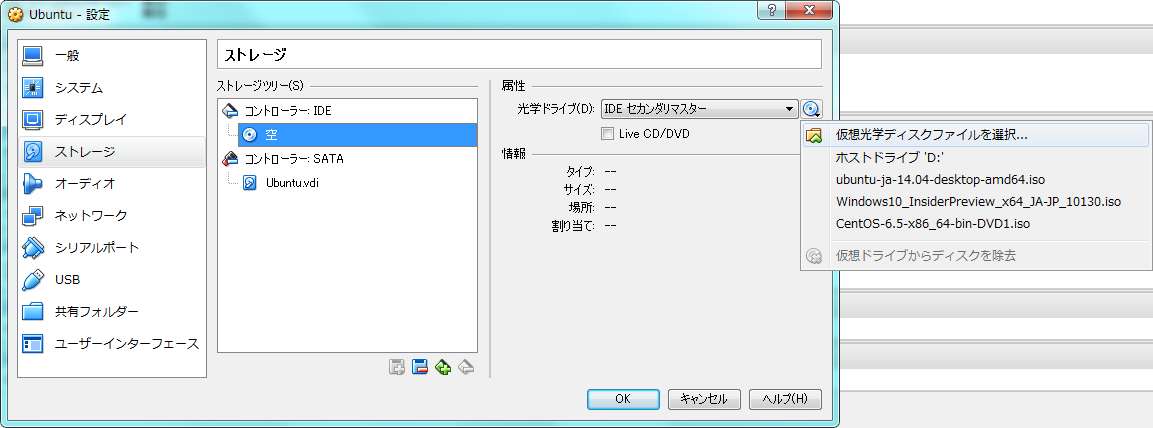
\includegraphics[width=15cm]{iso_set.png}
	\caption{ISOイメージのマウント}\label{isoset}
	\end{figure}
	
	「OK」をクリックして「起動(T)」を押すとゲストマシンが起動し,Ubuntuのインストールウィザードが表示される.\\
	表示内容に従ってウィザードを進めていくと,ゲストマシン内にUbuntuがインストールされる.

	\begin{figure}[H]
	\centering
	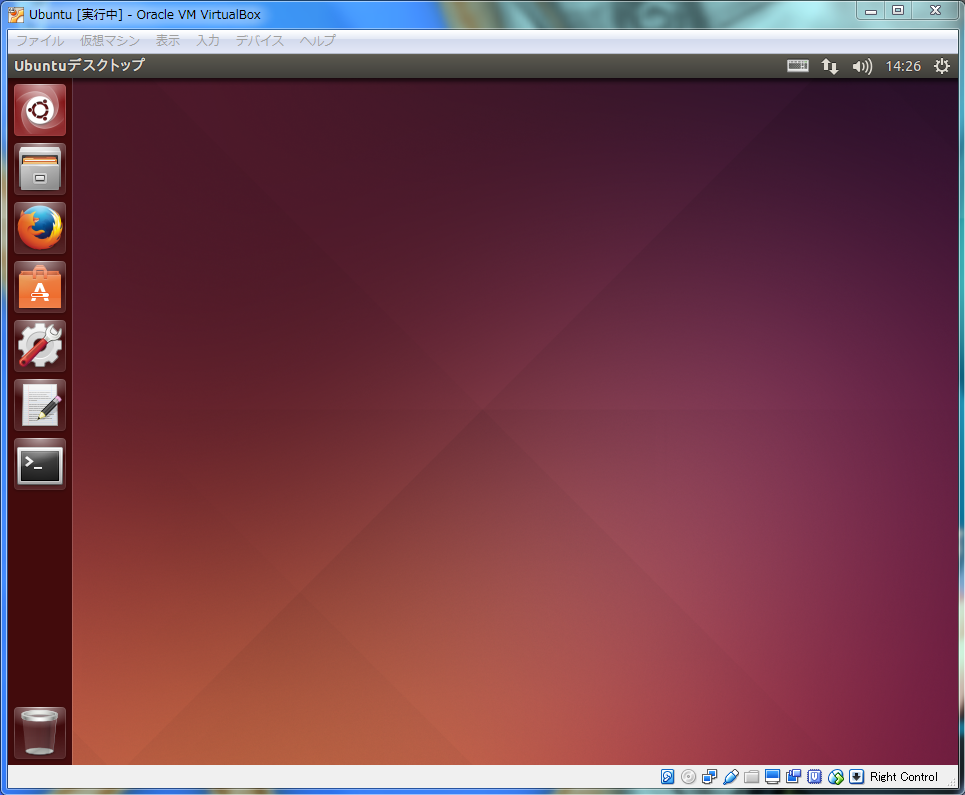
\includegraphics[width=15cm]{Ubuntu_on_VirtualBox.PNG}
	\caption{VirtualBox上で動作するUbuntu 14.04}\label{UbuntuVBox}
	\end{figure}

 \item[Guest Additionsのインストール]\mbox{}\\
	ゲストマシンにインストールしたUbuntuを立ち上げ,ホストOS側のメニューバーにある「デバイス」から「Guest Additions CD イメージの挿入...」を選択するとウィンドウが開く.\\
	「実行する(R)」を押してインストールし,Ubuntuを再起動するとGuest Additionsの機能が有効になる.
	
 \item[Tweepyのインストール]\mbox{}\\
	本研究では,Pythonというプログラム言語でTwitterを利用するためのライブラリであるTweepyをインストールした.\\
	Ubuntuのアプリケーション一覧より「端末」を開き,下記のコマンドを実行するとTweepyがインストールされる.
		
		\begin{lstlisting}[caption={}, label={}]
			sudo apt-get install python-setuptools python-pip
			sudo easy_install tweepy
		\end{lstlisting}
		
 \item[タイムラインの取得]\mbox{}\\
	本研究では,矢吹研究室に所属する3年生のうち,Twitterのアクティブユーザである4人の協力を得て,各々のマシンやTwitterアカウントを利用してTwitterタイムラインを取得した.\\
	所属する研究室の指導教員が自らのブログに記載した方法に則り,Streaming APIを利用してTwitterのタイムラインを取得する.方法は下記のとおりである.\\
	%ここに携帯番号登録の旨も書く
	Twitterにログインし,画面右上のアカウントアイコンをクリックするとプルダウンメニューが表示されるため,「設定」を選択する.\\
	
	\begin{figure}[H]
	\centering
	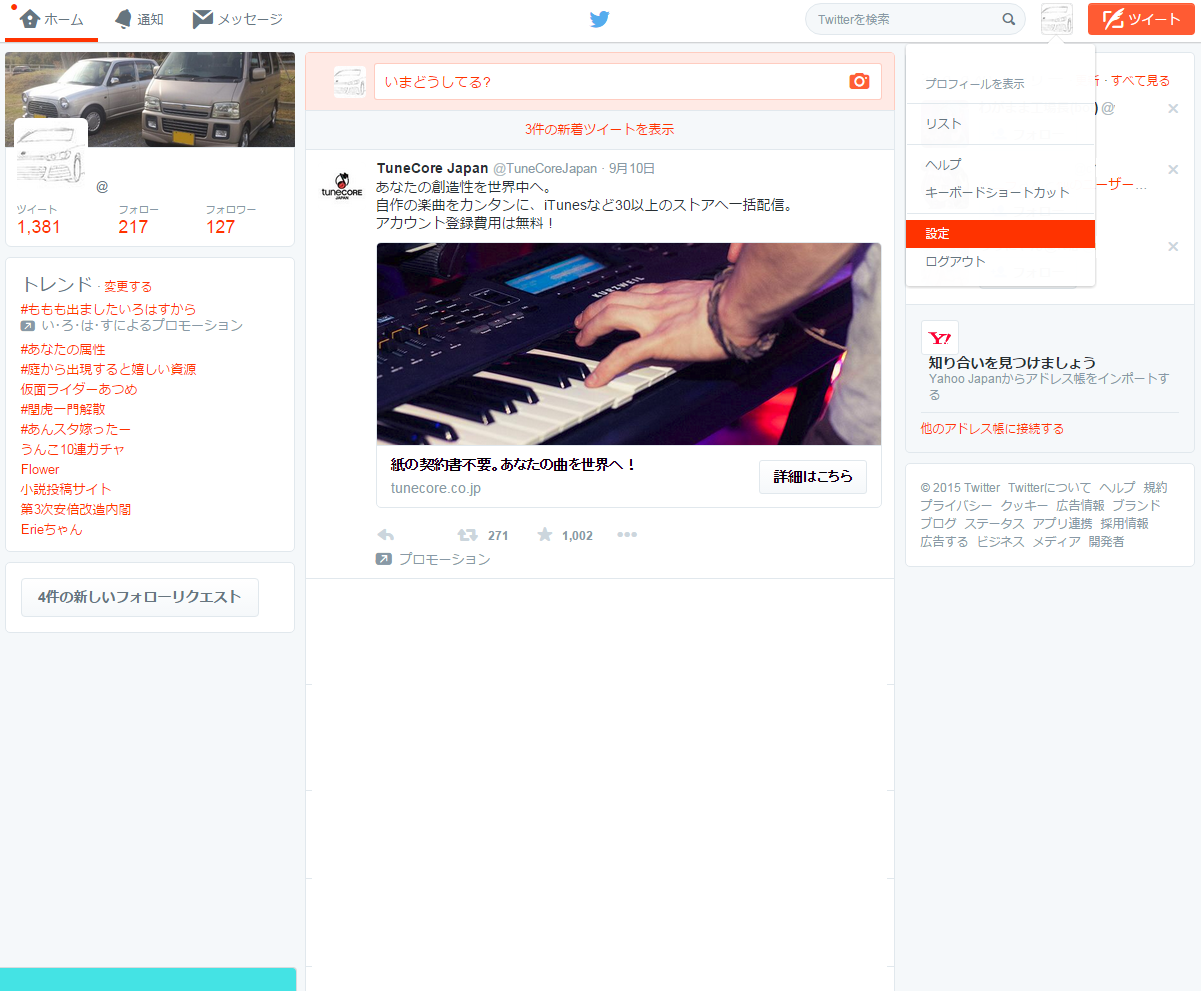
\includegraphics[width=15cm]{TwitterHome.png}
	\caption{プルダウンメニューの表示}\label{pulldown}
	\end{figure}
	
	左側のメニューより「モバイル」を選択し,携帯電話番号を入力して「続ける」をクリックする.
	
	\begin{figure}[H]
	\centering
	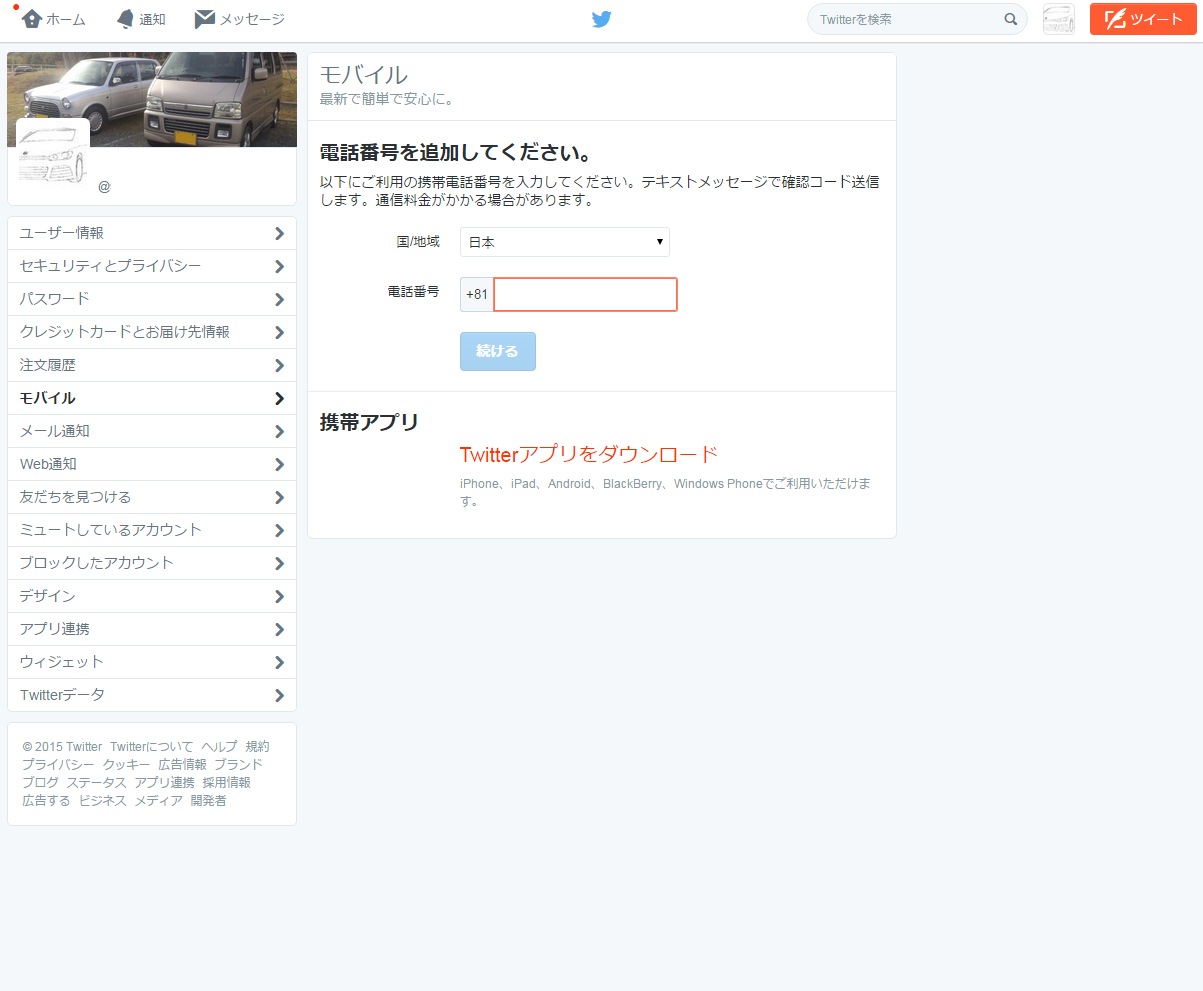
\includegraphics[width=15cm]{TwitterMobile1.png}
	\caption{携帯電話番号の入力画面}\label{mobile1}
	\end{figure}
	
	Twitterの開発者向けページ(https://dev.twitter.com)にアクセスし,画面下方にある「Manage Your Apps」(下図の赤枠で囲った部分)をクリックする.
	
	\begin{figure}[H]
	\centering
	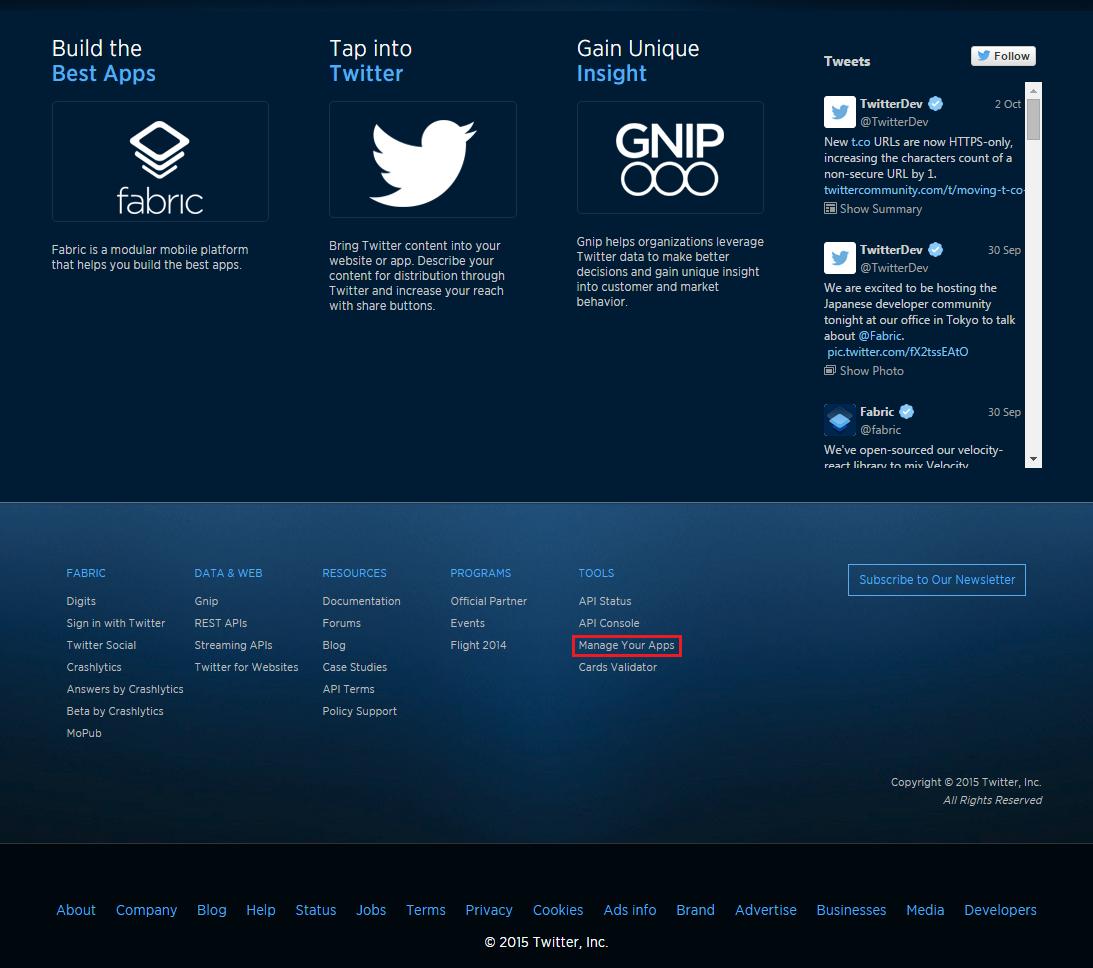
\includegraphics[width=15cm]{dev_twitter.PNG}
	\caption{Twitterの開発者向けページ}\label{devTwitter}
	\end{figure}
	
	「You don't currently have any Twitter Apps.」と表示されるので,その下にある「Create New App」をクリックし,アプリケーション作成画面に移る.\\
	「Name(アプリケーションの名前)」,「Description(アプリケーションの説明)」,「Website(アプリケーションを動かすWebサイトのトップページのURLを本来入力しなければならないが,そういったWebサイトがないため,ここでは各TwitterアカウントのプロフィールページのURLを記載しておく)」をそれぞれ入力し,規約に同意して「Create your Twitter application」をクリックするとアプリケーションが作成される.\\
	これにより,後述するプログラムに必要な情報(Consumer Key,Consumer Secret,Access Token,Access Token Secret)を取得することができる.\\
	ただし,Access TokenとAccess Token Secretに関してはアカウントごとに作成する必要があるため,それらを作成するためのWebサービスを用いる.\\
	http://getaccesstoken.herokuapp.com/にアクセスし,表示されたページの指示に従って作成したアプリケーションの設定を変更する.
	
	\begin{figure}[H]
	\centering
	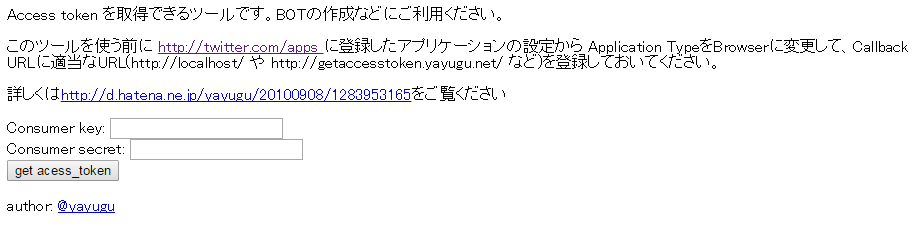
\includegraphics[width=15cm]{get_access_token.PNG}
	\caption{http://getaccesstoken.herokuapp.com/の表示}\label{getaccesstoken}
	\end{figure}
	
	変更が済んだら,ブラウザで予めAccess TokenとAccess Token Secretを取得したいアカウントでログインし,再び上記サイトにアクセスする.\\
	「Consumer key」,「Consumer secret」に自分のアカウントのそれぞれの情報を入力し,「get acess\_token」をクリックするとAccess TokenとAccess Token Secretが表示されるため,これらをメモしておく.\\
	「端末」に「python stream.py >> result.dat」と入力して下記のプログラム(stream.py)を実行する
	(consumer\_keyとconsumer\_secretはアプリケーション作成時に取得した自分のアカウントのそれぞれの情報を,access\_tokenとaccess\_token\_secretは各々のアカウントの情報を予め入力しておく).
		\begin{lstlisting}[caption={}, label={}]
			# -*- coding: utf-8 -*-
 
			from tweepy.streaming import StreamListener
			from tweepy import OAuthHandler
			from tweepy import Stream
 
			consumer_key = ""
			consumer_secret = ""
 
			access_token = ""
			access_token_secret = ""
 
			class StdOutListener(StreamListener):
    				def on_data(self, data):
        				if data.startswith("{"):
            					print data
        				return True
 
    				def on_error(self, status):
        				print status
 
			if __name__ == '__main__':
    				l = StdOutListener()
    				auth = OAuthHandler(consumer_key, consumer_secret)
    				auth.set_access_token(access_token, access_token_secret)
 
    				stream = Stream(auth, l)
    				stream.userstream()
		\end{lstlisting}



 \item[取得したタイムラインの処理]\mbox{}\\
	取得したタイムラインはJSON形式で保存されており(result.datというファイルに保存されている),この形式のままではつぶやきを閲覧したり,分析することができない.\\
	そこで下記のparse.pyを用いて必要なデータだけを,正しく読める形にして抽出する.\\
	「端末」に「python parse.py 20151005000000 20151005235959 < result.dat」と入力して実行すると,日本時間の2015年10月5日00時00分00秒から2015年10月5日23時59分59秒のつぶやきの本文のみが抽出され,「端末」上に表示される.\\
	parse.pyのソースコードは以下のとおりである.
		\begin{lstlisting}[caption={}, label={}]
			#!/usr/bin/env python
			import sys, json, time, calendar
			#from pprint import pprint
 
			def YmdHMS(created_at):
				time_utc = time.strptime(created_at, '%a %b %d %H:%M:%S +0000 %Y')
				unix_time = calendar.timegm(time_utc)
				time_local = time.localtime(unix_time)
				return int(time.strftime("%Y%m%d%H%M%S", time_local))
 
			argv = sys.argv
			start_time = 0
			end_time = 99999999999999
			if 1 < len(argv):
				start_time = int(argv[1])
				end_time = int(argv[2])
 
			for line in sys.stdin:
				try:
					tweet = json.loads(line)
        				#pprint(tweet)
            					tweet_time = YmdHMS(tweet['created_at'])
            					if start_time <= tweet_time and tweet_time <= end_time:
                					tweet_sec = tweet_time-start_time
                					screen_name = tweet['user']['screen_name']
                					text = tweet['text'].encode('utf-8')
                					url = "https://twitter.com/#!/%s/status/%s"\
                    						% (screen_name, tweet['id_str'])
                					#print tweet_sec, url, text
                					#print text
                					t = time.strptime(str(tweet_time), "%Y%m%d%H%M%S")
                					print time.strftime("%H:%M:%S", t), text
    				except StandardError:
        				pass
		\end{lstlisting}
 \item[タイムラインの分析]\mbox{}\\
	上記手順で抽出したつぶやきはテキストエディターにコピー\&ペーストし,テキストファイルとして保存する.\\
	UserLocalテキストマイニング(http://textmining.userlocal.jp/)にアクセスし,「テキストファイルを解析」の「解析ページへ」をクリックする.\\
	保存したテキストファイルを選択し,「解析する」をクリックすると解析結果が表示される.なお,一度に解析できる文字数は100,000文字までである.
	
\end{description}
		
\chapter{結果}

\chapter{考察}

\chapter{結論}

\bibliographystyle{junsrt}
\bibliography{biblio}%「biblio.bib」というファイルが必要.

\end{document}